\documentclass[times, utf8, zavrsni, numeric]{fer}
\usepackage{booktabs}

\begin{document}

\thesisnumber{2324}

\title{Orthobalancer: aplikacija za kreiranje skupova bioloških vrsta usporedive taksonomijske širine}

\author{Ivan Slijepčević}

\maketitle

% Ispis stranice s napomenom o umetanju izvornika rada. Uklonite naredbu \izvornik ako želite izbaciti tu stranicu.
\izvornik

% Dodavanje zahvale ili prazne stranice. Ako ne želite dodati zahvalu, naredbu ostavite radi prazne stranice.
\zahvala{
zahvale
}

\begin{sloppypar}
\tableofcontents
\end{sloppypar}

\listoffigures
\listoftables

\chapter{Uvod}
\label{chap:uvod}


automatizacija (posla kroz cjevovod->treba ići u neko uvodno poglavlje o namjeri)

robusnost

\chapter{Teoretski uvod}
\label{chap:teoretski-uvod}

\section{Homologija proteina}
\label{sec:homologija}

Homologija u biološkom smislu predstavlja slične osobine među vrstama na
različitim razinama organizacije života, poput organa, tkiva, stanice ili
molekule. Homologne osobine uočene među jedinkama različitih vrsta obično
upućuju na zajedničke pretke tih vrsta u evoluciji. Međutim, u molekularnoj
biologiji termin homolog se često koristi i za naznačavanje sličnosti. bez
obzira na genetsko srodstvo.\cite{bioinfo1}

\begin{figure}[h!]
\centering
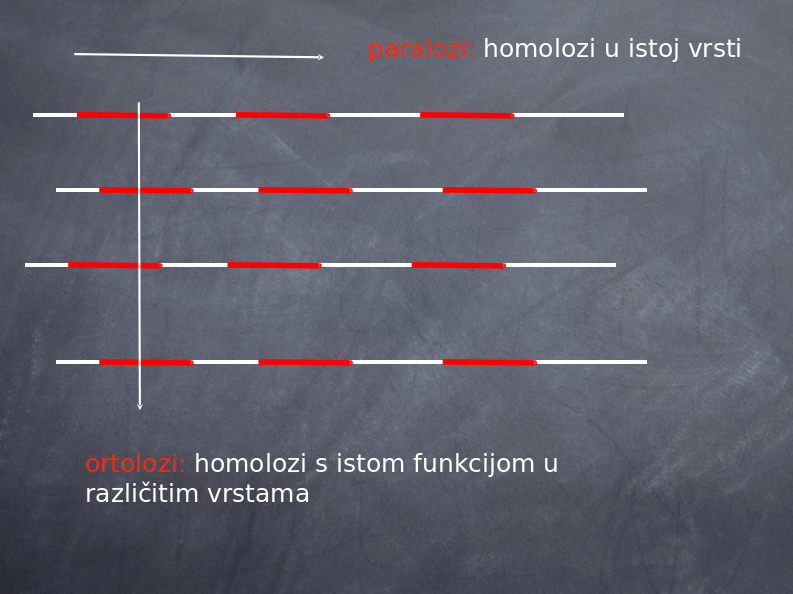
\includegraphics[width=4.5in]{figures/ortho-para.png}
\caption{Vizualni prikaz ortolognih i paralognih gena na genetskim lancima
raznih vrsta}
\label{fig:para-ortho}
\end{figure}

Za homologne sekvence proteina kažemo da su ortologne kad su direktni
potomci neke sekvence u zajedničkom pretku, bez da su prošle duplikaciju
gena. Drugim riječima, ortologne sekvence se mogu naći u jedinkama
različitih vrsta, a obavljaju istu funkciju u svim tim vrstama. Paralogne
sekvence su homologne sekvence koje su nastale od dvije različite kopije
nekog gena koji je prošao kroz proces duplikacije gena u nekom zajedničkom
evolucijskom pretku. Paralozi se mogu naći u jedinkama jedne ili više vrsta te
ne obavljaju nužno identične funkcije. Slika \ref{fig:para-ortho} predočuje
razliku paraloga i ortologa.




\chapter{Podaci}
\label{chap:podaci}

Orthobalancer radi sa primarnim proteinskim strukturama --- sekvencama
reziduuma, odnosno aminokiselina. Za zapis sekvenci koristi se standardizirani
FASTA format. Orthobalancer za svoj rad koristi dvije
NCBI-jevih\footnote{National Center for Biotechnology Information} baza
podataka od kojih jedna sadrži sekvence formatirane u FASTA format, a druga
taksonomsko stablo živog svijeta.


\section{FASTA format}
\label{sec:fasta}


\section{Neredundantna baza}
\label{sec:nrdb}


\section{Taksonomsko stablo živog svijeta}
\label{sec:taxdb}


\section{Ulaz}
\label{sec:input}

Aplikacija kao ulaz prima nekolicinu paralognih proteina u FASTA formatu. Ako
korisnik posjeduje samo sekvencu proteina, može ju zadati bez FASTA zaglavlja,
no u tome je slučaju dužan dati ime unesenoj sekvenci. Nužno je imati ime za svaki
ulazni paralog te je nužno da da su sva međusobno jedinstvena.

Dodatno, korisnik može specificirati čvorove taksonomskog stabla za čija
podstabla smatra da sadrže zamjenjive vrste. Ponuđen je i osnovni skup
zamjenskih čvorova za koje se vjeruje da bi mogli biti od koristi korisniku.


\section{Izlaz}
\label{sec:output}

Web aplikacija za završetak izvođenja prikazuje tablicu balansiranih vrsta.
Stupci tablice su imenovani po paralozima s ulaza. Retci su grupirani u
zamjenske čvorove. Svaki redak predstavlja jedan balansirani skup vrsta. U
stupcu pod pojedinim paralogom nalazi se ortologna vrsta, a lijevo od svih vrsta
je zapisan čvor na kojem su vrste tog retka balansirane. Primjer tablice se može
vidjeti naslici \ref{fig:tablica}.

\begin{figure}[h!]
\centering
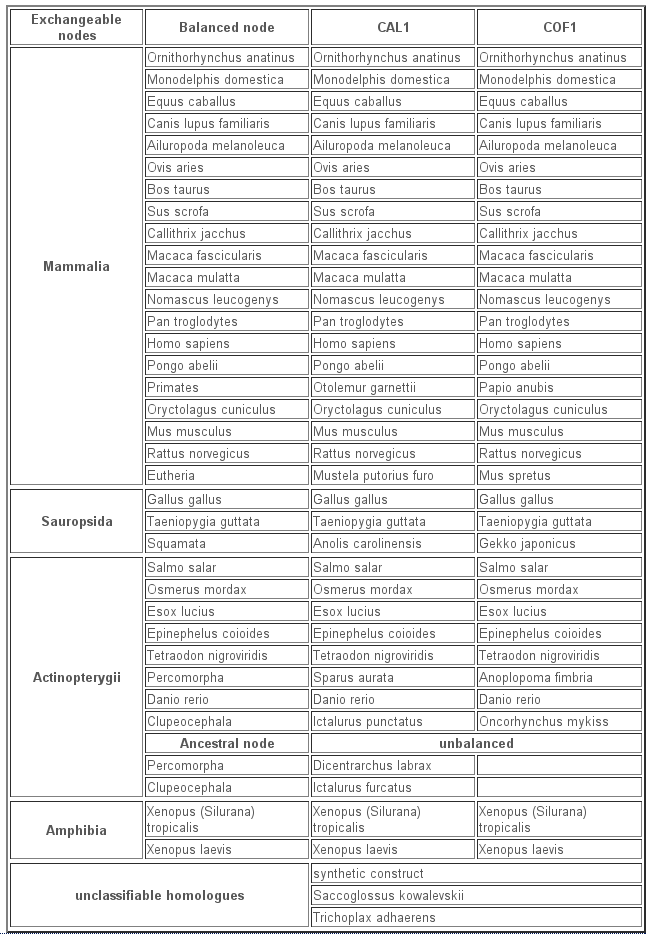
\includegraphics[width=4.75in]{figures/tablica.png}
\caption{Izlazna tablica sa web stranice Orthobanalcera}
\label{fig:tablica}
\end{figure}

Također, završna stranica sadrži poveznice za preuzimanje generiranih datoteka
tijekom izvođenja. Datoteke su opisane u nastavku.

\chapter{Metode}
\label{chap:metode}

pipeline neki dijagram za pipeline (sequence / activity / state)

tax dio pseudokod

neki sequence dijagram za sve

izlaz

(prebaciti u neki teex file za server) server slike (ulaz, zamjenjivi, izvršavanje, kraj, error)

\chapter{Implementacija}
\label{chap:implementacija}

% todo ozbiljno razmisliti sto i kamo sa ovim tekstom. ne zasluzuje cijelo
% poglavlje

Aplikacija je pisana u programskom jeziku Python verzije 2.7. Aplikacija se
dijeli u nekoliko zasebnih cjelina. U središtu aplikacije nalazi se cjovovod
koji poziva alate poput BLAST-a\cite{altschul1997gapped} i fastacmd-a za
komuniciranje sa NCBI-jevom neredundantnom bazom, zatim dio aplikacije za
odabir i balansiranje vrsta na taksonomskom stablu te alat mafft\cite{mafft} za
poravnanje sekvenci. Rad cjevovoda detaljo je opisan u poglavlju
\ref{chap:cjevovod}, a modul za odabir i balansiranje vrsta u poglavlju
\ref{chap:tax}. Pored cjevovoda implementirana je mrežna aplikacija kao
korisničko sučelje za cijeli program. Mrežna aplikacija je implementirana
koristeći Flask microframework verzije 0.7, dok su operacije na klijentskoj
strani implementirane u javascriptu uz korištenje biblioteke jQuery. Opis rada
mrežne aplikacije dan je u poglavlju \ref{chap:server}.



\chapter{Rezultati}
\label{chap:rezultati}

\chapter{Zaključak}
\label{chap:zakljucak}

Orthobalancer nudi jedinstven i izravan način odabira skupova ortolognih
proteinskih sekvenci iz bliskih taksonomskih grana. Aplikacija prima nekoliko
paralognih proteinskih sekvenci, a vraća skup ortologa za svaki paralog uz
informaciju koliko je pojedini ortolog evolucijski udaljen od ortologa iz
skupova ostalih paraloga.

Aplikacija je izrađena kao mrežna aplikacija te je dostupna na URL-u
\footnotesize{\url{http://orthobalancer.bmad.bii-sg.org}}. \normalsize
Mrežna aplikacija izrađena je robusno, a unošenje podataka dinamički je
prilagodivo potrebama korisnika.

Aplikacija u pozadini radi na razini vrsta i taksonomske hijerarhije umjesto na
razini proteinskih sekvenci. Iako takav pristup nema garanciju da su pronađene
sekvence doista ortologne, prednost nad konvencionalnim metodama jest u tome što
je pokriven znatno veći broj proteina i vrsta. Klasične metode rade samo na
potpuno sekvenciranim genomima kakvih je općenito malo, ograničeni su u glavnom
na kralježnjake, a sekvenciranje cijelog genoma je sklono pogreškama.
Orthobalancer doprinosi kreiranju potrebnih balansiranih skupova sekvenci za
organizme za koje potpun genom nije poznat.

Za daljnje istraživanje, ideja zajedničkog podskupa vrsta među vrstama
usporedive taksonomske širine bi se mogla probati primijeniti za drugačije
namjene.



\bibliography{literatura}
\bibliographystyle{fer}

\begin{sazetak}

% OrthoBalancer mrežna aplikacija za ulaz uzima skup od $n$ \emph{bona fide}
paralognih --- sličnih, ali kodiranih različitim genom --- proteinskih sekvenci
iz iste vrste. Za svaki paralog, aplikacija vraća skup najsličnijih proteina iz
drugih vrsta prisutnih u ishodišnoj bazi podataka. U jezgri aplikacije je modul
koji koristi taksonomsko stablo živog svijeta kako bi pronašao zajednički
podskup $n$ skupova vrsta, ali ipak dozvoljavajući razinu neizrazitosti ili
``zamjenjivosti" srodnih vrsta. Stupanj zamjenjivosti, odnosno razina u
taksonomskom stablu ispod koje bilo koja vrsta može poslužiti kao reprezentant
pripadajućeg podstabla, se može podesiti od strane korisnika.


\kljucnerijeci{}
\end{sazetak}

\clearpage

\engtitle{Orthobalancer: web application for creation of taxonomically balanced sets of orthologous protein sequences}
\begin{abstract}

% OrthoBalancer web application takes as an input a set of  $n$ \emph{bona fide}
paralogous --- similar, but encoded by a different gene --- protein sequences from
the same species. For each of the paralogues, the application returns the set of
the most similar proteins from other species present in the underlying database.
At its core is a module that uses taxonomic tree to find a common subset of $n$
sets of species, while allowing some fuzziness or ``exchangeability'' of related
species.  The degree of exchangeability, that is, the level in the taxonomic
tree below which any species can serve as a representative of the branch, can be
modified by the user. 


\keywords{}
\end{abstract}

\end{document}
